\subsection{Architektur} \label{sec:ArchitekturV1}
    Für die Umsetzung der Anforderungen sind verschiedene Komponenten in der Umsetzung der \ac{API} nötig:
    \begin{enumerate}
        \item \textbf{Framework} \label{arch_1}\\
            Um eine \ac{API} zu entwickeln, muss ein passendes Framework genutzt werden.
            Dadurch, dass keine Notwendigkeit für ein Frontend besteht gibt es hier wenig Eingrenzungen.
            \\
            Aus Erfahrungsgründen wurde das C\# Framework ASP.NET\textsuperscript{\cite{link:ASPNET}} gewählt.
            Mit diesem lassen sich unter anderem \ac{API}-Services bauen.
            Mittels der für das .NET Framework explizit vorhandenen IDE \glqq Visual Studio\grqq~bestehen auch native Debugging-Möglichkeiten.
            Durch die große und aktive Community von ASP.NET ist dieses Framework sehr gut dokumentiert und es existieren viele Open-Source-Bibliotheken.
        \item \textbf{Datenbank} \label{arch_2}\\
            Da für die beliebtesten JavaScript-Repositories durchschnittlich $2.429,9$ Abhängigkeiten bestehen (siehe Appendix \ref{sec:PackageMeanPopGitJsRepos}) sind durch die Menge dieser alle \ac{CVE}-Daten lokal zu persistieren, welche zu durchsuchen sind.
            Diese Daten dienen als Grundlage der Identifizierung von Schwachstellen in Paketen innerhalb von Projekten.
            Durch die oft große Anzahl der Abhängigkeiten eines Projektes ist die Anzahl der Lesezugriffe und deren Geschwindigkeit zu betrachten.
            Wichtig sind hier schnelle Lesezugriffe, da diese beim Abfragen der Datenbank die größte Laufzeiteinsparung bringen.

            Durch die Wahl des Frameworks auf ASP.NET ist es möglich einen \textit{embedded NoSQL-Document-Store} -- LiteDB zu nutzen. % TODO: https://www.litedb.org/
            Diese ist leicht intern nutzbar und muss als \textit{file-based DB} nicht separat explizit gestartet und verwaltet werden, womit diese auch im Container der \ac{API} mit enthalten ist.
        \item \textbf{Controller} \label{arch_3}\\
            Controller einer \ac{API} nehmen HTTP-Anfragen entgegen und reagieren darauf.
            Hier wird die Hauptaufgabe der \ac{API} geschehen, da alle Funktionalitäten, sei es Datenbankabfragen, Klonen eines zu untersuchenden Repositories oder die Untersuchung dieses, in einem solchen implementiert oder aufgerufen werden müssen.

            Notwendig sind hier vier Controller.
            (\hyperref[api_controller:one]{1}) Es muss ein Git-Controller zum nutzen von \ac{CVE}-Daten sowie zum Erhalt von zu analysierenden Repositories entstehen.
            In diesem sind Endpunkte zum Clonen des \ac{CVE}-Daten-Repositories sowie zum Clonen des Analyse-Repositories zu implementieren. % TODO: clone CVE-DATEN-REPO-LINK
            \\
            Weiterhin ist (\hyperref[api_controller:two]{1}) ein Controller für Abhängigkeiten nötig, in dem man aus dem zu analysierenden Repository den Abhängigkeitsbaum extrahiert sowie diesen mit Schwachstellendaten anreichert.
            \\
            Für die Untersuchung einzelner Pakete und Listen dieser ist ein weiterer (\hyperref[api_controller:three]{3}) Endpunkt zu implementieren.
            In diesem ist auch die Update-Funktion der Datenbasis hinzuzufügen.
            \\
            Weiterhin muss in jedem Endpunkt (\hyperref[api_controller:four]{4}) bei korrekter Antwort ein Context mitgeliefert werden, damit der gelieferte Inhalt so durch \ac{JSON-LD} zu interpretieren ist.
            Ebenfalls sind durch einen Controller die Rückgabedaten zu dokumentieren.
            Dazu ist zwischen Softwarepaketen und \ac{CVE}-Einträgen zu unterscheiden.
        \item \textbf{Datenmodelle} \label{arch_4}\\
            Um Daten korrekt in die Datenbank einzufügen, um ein Resultat-\ac{JSON} zu erzeugen oder die Paketliste intern zu verarbeiten -- dazu sind Datenmodelle nötig.
        \item \textbf{Konvertierung von und in JSON} \label{arch_5}\\
            Beim Einlesen der \ac{CVE}-Daten in die Datenbank ist eine Konvertierung vom vorhandenen \ac{JSON}-Format in Einträge der Datenbank vorzunehmen.
            Die aus der Datenbank genutzten, durch den Controller verarbeiteten, Daten müssen nun schließlich im \ac{JSON}-Format dem Benutzer übermittelt werden.
            \\
            Dies muss in den jeweiligen Controllern geschehen.
            Damit die Daten besser weiterverwendbar sind muss zusätzlich ein Kontext \glqq @context\grqq~hinzugefügt werden.
        \item \textbf{Rückgabetypen} \label{arch_5_1}\\
            Da eine REST-konforme \ac{API} implementiert werden soll, müssen die Rückgabetypen dem HTTP-Protokoll entsprechen.
        \item \textbf{Container} \\
            Um die \ac{API} unabhängig von der Umgebung zu nutzen muss die Anwendung in einem Container, zum Beispiel Docker, Kontext gestartet werden.
            Für den Bau der Containers wird eine \textit{docker-compose.yml} (siehe Appendix \ref{sec:dockerComposeYml}) genutzt.
    \end{enumerate}
    Weiterhin muss das \ac{JSON-LD}-Format für die Rückgabedaten definiert werden (Forschungsfrage \ref{q:three}).
    \\ \\ 
    \noindent Die endgültige Architektur hat folgenden Aufbau:
    \begin{figure}[H]
        \centering
        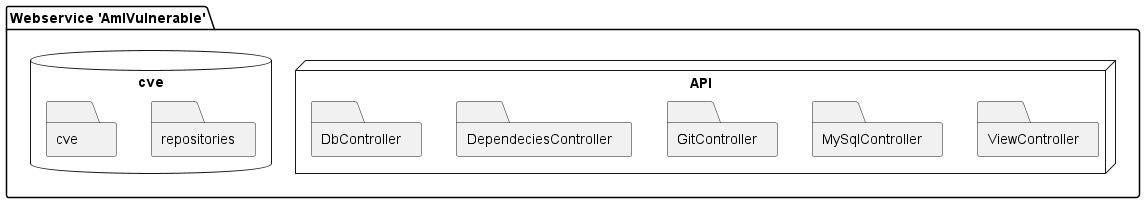
\includegraphics[width=0.95\textwidth]{5_concept/architecture.png}
        \caption{Architektur des Webservices}
        \label{png:ArchitekturDesWebservices}
    \end{figure}
